\begin{flushleft}

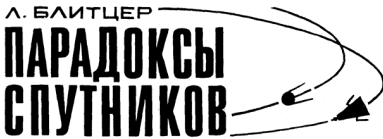
\includegraphics[width=\linewidth]{img/satellite.png}
\end{flushleft}

\vspace{15pt}


\leftskip=2cm \rightskip=1cm
\fontsize{12}{13}\selectfont
\begin{minipage}{14cm}
	\textbf{    Закон инерции хорошо известен. И хотя на Земле мы никогда не видели равномерно движущегося тела, на которое не действовали бы никакие силы, тем не менее шайба на льду может служить хорошей моделью такого тела: сила трения мала, а сила тяжести компенсируется силой реакции льда. В космосе, там, где летают искусственные спутники, ничто не компенсирует силу тяжести. Поэтому там тела, на которые не действуют никакие силы (кроме силы притяжения), движутся ло эллипсам, параболам или гиперболам. Это можно считать "законом инерции" для спутников$^1$  ).}
 
 \textbf{ \hspace{10mm} Как же выглядит для спутника второй закон Ньютона, то есть как изменяется скорость спутника, если на него действует какая-либо сила, кроме сил притяжения к Земле? об этом рассказано в статье, которую мы перепечатываем из "American Journal of Phisics" за 1971 г. Текст § 2 несколько изменен с тем, чтобы рассматривать движение не по эллипсу, а по окружности, так как формулы для такого движения можно легко получить, пользуясь школьным учебником физики. Эллиптичность орбиты спутника в данном случае несущественна.}
 
 \textbf{ \hspace{10mm}Статья подготовлена к печати Н. Я. Смородинской.}
\vspace{1cm}
\end{minipage}


\fontsize{14}{9}\selectfont
\begin{multicols}{2}

\leftskip=0.1cm \rightskip=1cm
\fontsize{14}{15}\selectfont
\begin{minipage}{8.5cm}
\begin{center}
\subsection*{1. Введение}
\end{center}
 \hspace{10mm}Как вы думаете, что просиходит со скоростью и кинетической энер-гией искусственного спутника Земли при торможении в атмосфере? Вы наверняка ошибетесь, если будете руководствоваться лишь тем, что вам подсказывает повседневный пземнойи опыт. Оказывается, скорость и ки-нетическая энергия спутника при торможении в атмосфере возрастают! Это удивительное явление было на-столько неожиданным, что его стали называть парадоксом. Мы расскажем 
\footnote{') См. статью А. К. К и к о и н а "Вращательное движение тел", "Квант" №1,1971. }
\end{minipage}


\fontsize{14}{8}\selectfont
\leftskip=0.5cm \rightskip=0.7cm
\begin{minipage}{8.5cm}
здесь о трех, казалось бы, совершенно разных явлениях, объяснение которых связано с этим парадоксом.
 
\begin{enumerate}
 \item Сокращение -размеров орбиты спутника и увеличение его скорости в земной атмосфере.
 \item Колебание экваториального спутника Земли относительно положения устойчивого равновесия.. 
\item Изменение продолжительности земного месяца. 
 \end{enumerate}
 \hspace{10mm}Первое из перечисленных явлений объясняется торможением в атмосфере, причина второго кроется в "трехосности" нашей планеты, а третье связано с тем, что на поверхности Земли образуются приливные выступы. 
\end{minipage}
\end{multicols}

\setlength{\columnsep}{0cm}
\twocolumn
\leftskip=0cm \rightskip=0cm
\fontsize{14}{10}\selectfont
\begin{minipage}{8cm}
\begin{center}
	\subsection*{II. Невозмущенная кеплеровская орбита}
\end{center}


\hspace{10mm}Давайте вспомним самые простые уравнения движемия,подчиняющегося законам Кеплера. Если бы Земля была сферически симметрична и если бы вокруг нее не было ни атмосферы, ни других возмущающихся факторов, то хорошо известно, что орбита земного спутника представляла бы собой эллипс, один из фокусов которого лежал бы в центре Земли (рис. 1). 

\hspace{10mm}Когда орбита спутника близка к окружности с радиусом а, то период обращения его вокруг Земли равен

\begin{equation}
T = 2\pi \sqrt{\frac{a^3}{\mu}}
\end{equation}
 где $\mu = \gamma M$ ($\gamma$ - гравитационная постоянная и М - масса Земли). 
 

\hspace{10mm}Согласно третьему закону Кеплера таким же будет и период обращения спутника по эллиптической орбите с большой полуосью, равной а. \hspace{10mm}Можно показать, что при движе-нии по круговой орбите потенциальная энергия U, кинетическая энергия К и полная энергия Е спутника выражается через а, $\mu$ и массу спутника $m$ следующим образом: 
\begin{equation}
  U = -\frac{\mu m}{a},	\footnote{) См. статью Н. М. С п е р а гг с к о г о .Потенциальная энергия тел в поле тяжести. на стр. 20. }
\end{equation} 
\begin{equation}
	K = \frac{\mu m}{2a},
\end{equation} 
\begin{equation}
	E = -\frac{\mu m}{2a}.
\end{equation} 
\end{minipage}

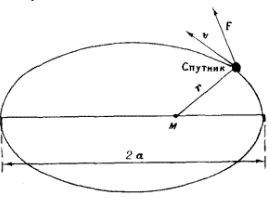
\includegraphics[width=200pt]{img/picture1.png}
\fontsize{12}{8}\selectfont
\textbf{\\Рис.1.Кеплеровский эллипс.F-возмущающая сила.}

\leftskip=0.3cm \rightskip=1cm
\fontsize{14}{10}\selectfont
\begin{minipage}{8cm}
Отсюда видно, что эти величины связаны соотношением 
\begin{equation}
	U = -2K = 2E
\end{equation}
 Для эллиптической орбиты соотношение (5) и формулы (2)-(4) остаются верными, но вместо кинетической и потенциальной энергии нужно говорить о средней (за один оборот вокруг Земли) кинетической и средней потенциальной энергиях спутника. 

\begin{center} 
\textbf{III. Объяснение парадокса}
\end{center}
\hspace{10mm}Рассмотрим теперь, что происходит, когда на спутник действует какая-нибудь произвольная дополнительная сила. Очевидно, что если эта сила больше гравитационной (равной $\frac{\mu}{r^2}$ ), то она должна играть основную роль. Это условие выполняется, например, в момент запуска спутника. Если же возмущающая сила мала по сравнению с силами гравитации, то орбита должна быть кеплеровской (то есть эллипсом или окружностью.) Именно этот случай мы и будем исследовать. \hspace{10mm}Любую непрерывно действующую возмущающую силу F можно заменить последовательностью бесконечно малых импульсов. В результате работы, совершаемой силой F в течение произвольного малого интервала времени $\Delta t$, энергия спутника возрастает на величину $\Delta E$:
 \begin{equation}
 	\Delta E = F_T \Delta S = F_T \nu \Delta t,
 \end{equation}
  
 где $F_T$ - тангенциальная составляющая силы F, направленная по касательной к орбите, а v - скорость спутника. Бесконечно малому приращению энергии $\Delta E$ соответствует увеличение радиуса орбиты спутника на бесконечно малую величину $\Delta a$. Посмотрим теперь на формулу (4). Мы увидим, что с увеличением энергии спутника радиус его орбиты увеличивается. Сосчитаем, на какую величину $\Delta a$ изменится радиус 
\end{minipage}

\leftskip=0cm \rightskip=0cm
\fontsize{14}{10}\selectfont
\begin{minipage}{8cm}
	
	
	орбиты, если энергия спутника изменится на $\Delta E$.
	
	
	\begin{equation}
		E = - \frac{\mu m}{2a}; E + \Delta E = - \frac{\mu m}{2(a + \Delta a)},
	\end{equation}
	отсюда
	\begin{equation}
		\frac{\Delta E}{E} = - \frac{1}{1 + \frac{a}{\Delta a}} \approx -\frac{\Delta a}{a}
	\end{equation}
	или
	\begin{equation}
		\Delta a = - \frac{a}{E}  \Delta E = \frac{2a^2}{\mu m} \Delta E
	\end{equation}
	
	
	\hspace{10mm}Найдём ещё связь между изменением скорости и изменением кинетической энергии 
	\begin{equation}
		K + \Delta K = \frac{m (v + \Delta v)^2}{2}
	\end{equation} 
	и
	\begin{equation}
		\frac{\Delta K}{K} \approx  2 \frac{\Delta v}{v}
	\end{equation} 
	отсюда
	\begin{equation}
		\Delta v = \frac{v}{2} \frac{\Delta K}{K} = -\frac{v}{2K} \Delta E
	\end{equation} 
	т.к. из соотношения (5)
	\begin{equation}
		\Delta K = - \Delta E
	\end{equation}	
	Подставляем теперь значение $\Delta E = F_T v \Delta t$,получим 
	\begin{equation}
		\Delta v = - \frac{1}{m} F_T \Delta t.
	\end{equation} 
	Отсюда,считая v и t малыми, получим выражение для ускорения спутника
	\begin{equation}
		W = - \frac{1}{m} F_T
	\end{equation}
	
\end{minipage}

\leftskip=0cm \rightskip=0cm
\fontsize{14}{10}\selectfont
\begin{minipage}{10cm}
	\begin{flushright}
		\textbf{Таблица 1}
	\end{flushright}
	\begin{center}
		\begin{tabular}{ c |c| c| c }
			\hline
			Величина & Обозначение & \makecell{Если $\Delta E > 0$\\ (ускоряющая сила)} & \makecell{Если $\Delta E <0 $\\ (тормзящая сила)} \\ [0.5ex]
			\hline
			\makecell{Радиус орбиты\\(большая полуось в случае\\ движения по эллипсу)} & $a$ & увеличивается & уменьшается \\
			Период обращения & $T$ & увеличивается & уменьшается \\
			Кинетическая энергия & $K$ & уменьшается & увеличивается \\
			Потенциальная энергия & $U$ & увеличивается & уменьшается \\
			Линейная скорость & $v$ & уменьшается & увеличивается \\
		\end{tabular}
	\end{center}
\end{minipage}




\leftskip=0.3cm \rightskip=1cm
\fontsize{14}{10}\selectfont
\begin{minipage}{8cm}
	\hspace{10mm}Это уравнение на вид противоречит второму закону Ньютона (знак минус перед F). На самом деле никакого противоречия, конечно, нет, Вспомним, что сила F представляет собой лишь возмущение по сравнению с доминирующей силой $\frac{1}{r^2}$. Из формулы (10) видно, что если энергия спутника увеличилась из-за увеличения радиуса орбиты на $\Delta E$, то кинетическая энергия уменьшилась на $\Delta E$.
При этом потенциальная энергия увеличилась на $2\Delta E$, это и дало увеличение полной энергии.
	
	\hspace{10mm}Заметьте, что все наши рассуждения совершенно не зависят от того,какая именно возмущающая сила действует на спутник.
	
	\hspace{10mm}Исследуя зависимость всех. этих величин от знака $\Delta E$, можно составить таблицу 1. Из нее видно, что в результате возрастания орбитальной энергии спутника его период,потенциальная энергия и размеры орбиты растут, а линейная скорость уменьшается. Если же сила, действующая на спутник, уменьшает его	энергию, то это вызовет сокращение размеров орбиты и увеличение скорости.
	\begin{center}
		\textbf{IV. Торможение в атмосфере}
	\end{center}
	
	\hspace{10mm}Рассмотрим, что происходит при	торможении спутника в земной атмосфере. В этом случае возмущающая(тормозящая) сила направлена против движения, то есть $\Delta E$ всегда имеет отрицательный знак. В соответствии с таблицей 1 большая полуось и период обращения будут постепенно убывать,следовательно,средняя
	 
\end{minipage}


% Page 4 !!!


\leftskip=0cm \rightskip=0cm
\begin{minipage}{8cm}
	
	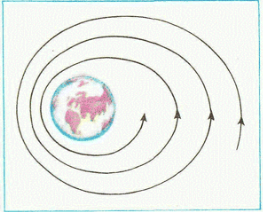
\includegraphics[width=230pt]{img/picture2.png}
	\fontsize{11}{8}
	\textbf{Рис. 2. Сжатие орбиты исскуственного спутника при торможении в атмосфере.}
	
	
	\fontsize{14}{10}\selectfont
	Скорость должна расти. Теряемая потенциальная энергия частично переходит в кинетическую,а остальная превращается в тепло. В перигее орбиты торможение максимально, потому что	в этой точке скорость и атмосферная плотность принимают свои максимальные значения. В апогее же торможение будет минимальным. Поскольку в перигее спутник каждый раз получает отрицательный импульс, его орбита будет постепенно сжиматься,все сильнее приближаясь к круговой(рис. 2). Такое сжатие орбиты спутника под действнем торможения в атмосфере,нензбежно для всех искусственных спутников Земли и обычно	сопровождается постепенным ростом скорости.Форма траектории приближается к окружности.
	

\begin{center}
	\textcolor{pink}{\textbf{V. Движение экваторнальных
	спутников с периодом 24 часа}}
\end{center}
	\hspace{10mm}Предположим, что Земля шарообразна, и рассмотрим искусственный спутник, который обращается в экваториальной плоскости по круговой орбите с периодом двадцать четыре часа. Поскольку движение спутинка по орбите пронсходнт синхронно с вращением Земли, географическая долгота такого спутника будет постоянной.
	
	\hspace{10mm}Ha этом свойстве основано использование спутников с круговыми орбитами для транслирования телевизионных
	
	
\end{minipage}


\leftskip=0.3cm \rightskip=1cm
\fontsize{14}{10}\selectfont
\begin{minipage}{8cm}
	передач и для географических
	исследований.
	
	\hspace{10mm}Ha самом деле распределение массы Земли неоднородно, а форма ee 	отличается от шарообразной, поэтому	внешнее гравитационное поле Земли похоже на гравитационное поле тела которое обладает тремя осями симметрии, а в сечении 
	экваториальной плоскостью имеет эллипс. (На основе данных, полученных при исследовании траекторий спутников, можно сказать, что разность длин большой и малой осей эллиптического экваторнального сечения Земли составляет	130 м, причем конец большой полуоси лежит на 15° западной долготы)
	
	\hspace{10mm}Давайте посмотрим, как происходит движение спутника во вращающейся системе отсчета, а именно в системе отсчета, связанной с Землей (рис. 3).Из соображений симметрии ясно, что когда спутник находится на продолжении одной из главных осей экваториального эллипса (в точках A
	или В), гравитационная сила ста
	
	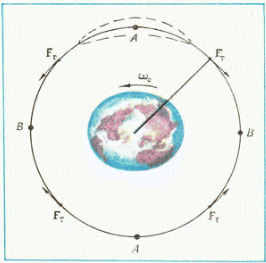
\includegraphics[width=230pt]{img/picture3.png}	
	\fontsize{10}{8}\selectfont
	\textbf{Рис. 3. Сечение Земли экваториальной плоскостью, перпендикулярной оси вращения(южный полюс находится за плоскостью рисунка).$F_T$ - сила, действующая на ступник вдоль касательной; A - положение устойчивого равновесия. B - положение неустойчивого равновесия. Пунктирной прямой показана траектория колебаний 24-часового спутника около положения устойчивого равновесия.}
	
\end{minipage}


% Page 5



\leftskip=0cm \rightskip=0cm
\fontsize{14}{10}
\begin{minipage}{8cm}
	новится чисто радиальной. Следовательно, в этих точках во вращающейся системе отсчета спутник должен быть в равновесии (висеть на месте). Во всех же остальных точках. спутник будет испытывать притяжение, направленное в сторону ближайшего конца. главной оси.Следовательно, будет существовать тангенциальная компонента силы $F_T$, направленная по касательной в сторону ближайшего конца главной оси (рис. 3)	На первый. взгляд может показаться,	что спутник должен получать ускорение в направлении действия силы $F_T$, однако, согласно уравнению (12),всё происходит совершенно иначе.В соответствии с разобранным парадоксом спутник будет медленно перемещаться в противоположном направлении в сторону ближайшего положения равновесия A, расположенного на малой оси. Поскольку спутник обладает некоторым количеством движения, он пройдет немного далыше точки A, после чего направление действия силы изменится на противоположное и спутник начнет постепенно	двигаться в обратную сторону. Таким. образом, спутник будет совершать колебания относительно положения равновесия А на малой оси.В этом процессе потери энертии не происходнт. Траектория спутника с периодом обращения 24 часа узображена пунктиром на рисунке 3.Период кодебаний зависнт от амплитуды, которая в свою очередь определяется начальными условиями.
	
	\begin{center}
		\textcolor{pink}{\textbf{VI. Увеличение длительности земного месяца}}
	\end{center}
	
	Перейдём к третьей задаче также связанной с рассмотреным парадоксом.Астрономам давно известно,что Луна постепенно удаляется от Земли, в результате чего период её обращения, то есть наш земной месяц, всё время увеличивается. Одним из следствий лунного притяжения являются происходящие на Земле приливы. Если бы вся Земля была покрыта океаном и между массой воды и морским дном
	
\end{minipage}


\leftskip=0.3cm \rightskip=1cm
\begin{minipage}{8cm}
	
	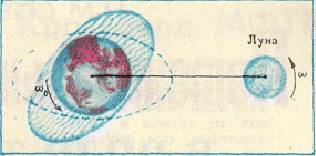
\includegraphics{img/picture4.png}
	\fontsize{10}{8}\selectfont
	\textbf{Рис. 4. Приливные выступы на Земле. (Для наглядности их размер сильно преувеличен)}
	
	\fontsize{14}{10}\selectfont
	нe было трения, то оба приливных горба лежали бы на прямой, соединяющей центры Луны и Земли (рис. 4).Однако скорость вращения Земли больше, чем угловая скорость движения Луны по орбите, поэтому приливные горбы из-за трения между морским дном и водой вытягиваются вперед по направлению вращения Земли.
	
	\hspace{10mm}Поверхность Земли и океанов, как показано на рисунке 4, приобретает форму эллипсоида, аналогичного экваториальному эллипсу предыдущей	задачи. Однако в этом случае водяной горб на Земле лишь немного опережает Луну. Горб, ближайший к Луне, взаимодействует с ней сильнее,чем более удаленный горб, поэтому	тангенциальная составляющая силы, действующей на Луну, направлена в ту сторону, в которую движется Луна
		
	\hspace{10mm}Орбитальная энергия Луны при этом возрастает, так как $F_T > 0$ Призвав на помощь все тот же парадокс, сразу заключаем, что полуось а Лунной орбиты и период обращения Луны вокруг Земли возрастают. Иными словами, Луна постепенно удаляется от Земли, a продолжительность месяца увеличивается. В то же время линейная и угловая скорости Луны уменьшаются.
	
	\hspace{10mm}Полный момент количества движения системы должен сохраняться,потому что дополнительное поступление энергии извне отсутствует. Раз момент количества движения Луны относительно центра Земли возpaстает, момент количества движения Земли относительно своей оси вращения должен все время убывать и день должен становиться длиннее.	
\end{minipage}